
%%--------------------------------------------------
%% Serway: Physics for Scientists and Engineers
%%--------------------------------------------------


%% Chapter 02: Motion in One Dimension
%%--------------------------------------------------


%% Table of Contents
%%--------------------------------------------------

%% 2.1 Position, Velocity, and Speed
%% 2.2 Instantaneous Velocity and Speed
%% 2.3 Analysis Models: The Particle Under Constant Velocity
%% 2.4 Acceleration
%% 2.5 Motion Diagrams
%% 2.6 The Particle Under Constant Acceleration
%% 2.7 Freely Falling Objects
%% 2.8 Kinematic Equations Derived from Calculus


%% Serway Multiple Choice Questions
%%--------------------------------------------------
\element{serway-mc}{
\begin{question}{serway-ch02-q01}
    The position of a particle moving along the $x$ axis is given by
    \begin{equation*}
        x = \left(21 + 22 t - 6.0 t^2\right)\, \si{\meter},
    \end{equation*}
    where $t$ is in seconds.
    What is the average velocity during the time interval
        $t = \SI{1.0}{\second}$ to $t = \SI{3.0}{\second}$?
    \begin{multicols}{2}
    \begin{choices}
        \wrongchoice{\SI{-6.0}{\meter\per\second\squared}}
        \wrongchoice{\SI{-4.0}{\meter\per\second\squared}}
      \correctchoice{\SI{-2.0}{\meter\per\second\squared}}
        \wrongchoice{\SI{-8.0}{\meter\per\second\squared}}
        \wrongchoice{\SI{+8.0}{\meter\per\second\squared}}
        %% NOTE: added for symmetry
        \wrongchoice{\SI{+2.0}{\meter\per\second\squared}}
    \end{choices}
    \end{multicols}
\end{question}
}

\element{serway-mc}{
\begin{question}{serway-ch02-q02}
    A bullet is fired through a board, \SI{14.0}{\centi\meter} thick,
        with its line of motion perpendicular to the face of the board.
    If it enters with a speed of \SI{450}{\meter\per\second} and emerges with a speed of \SI{220}{\meter\per\second},
        what is the bullet's acceleration as it passes through the board?
    \begin{multicols}{2}
    \begin{choices}
        \wrongchoice{\SI{-500}{\kilo\meter\per\second\squared}}
      \correctchoice{\SI{-550}{\kilo\meter\per\second\squared}}
        \wrongchoice{\SI{-360}{\kilo\meter\per\second\squared}}
        \wrongchoice{\SI{-520}{\kilo\meter\per\second\squared}}
        \wrongchoice{\SI{-275}{\kilo\meter\per\second\squared}}
    \end{choices}
    \end{multicols}
\end{question}
}

\element{serway-mc}{
\begin{question}{serway-ch02-q03}
    The position of a particle moving along the $x$ axis is given by
    \begin{equation*}
        x = 6.0 t^2 - 1.0 t^3,
    \end{equation*}
        where $x$ is in meters and $t$ in seconds.
    What is the position of the particle when it achieves its maximum speed in the positive $x$ direction?
    \begin{multicols}{3}
    \begin{choices}
        \wrongchoice{\SI{24}{\meter}}
        \wrongchoice{\SI{12}{\meter}}
        \wrongchoice{\SI{32}{\meter}}
      \correctchoice{\SI{16}{\meter}}
        \wrongchoice{\SI{2.0}{\meter}}
    \end{choices}
    \end{multicols}
\end{question}
}

\element{serway-mc}{
\begin{question}{serway-ch02-q04}
    The velocity of a particle moving along the $x$ axis is given for $t > 0$ by
    \begin{equation*}
        v_x = \left( 32.0 t - 2.00 t^3 \right)\,\si{\meter\per\second},
    \end{equation*}
        where $t$ is in seconds.
    What is the acceleration of the particle when (after $t = 0$) it achieves its maximum displacement in the positive $x$ direction?
    \begin{multicols}{2}
    \begin{choices}
      \correctchoice{\SI{-64.0}{\meter\per\second\squared}}
        \wrongchoice{zero}
        \wrongchoice{\SI{+128}{\meter\per\second\squared}}
        \wrongchoice{\SI{+32.0}{\meter\per\second\squared}}
        \wrongchoice{\SI{-32.0}{\meter\per\second\squared}}
    \end{choices}
    \end{multicols}
\end{question}
}

\element{serway-mc}{
\begin{question}{serway-ch02-q05}
    The position of a particle as it moves along the $x$ axis is given for $t > 0$ by
    \begin{equation*}
        x = \left( t^3 - 3 t^2 + 6 t \right)\,\si{\meter},
    \end{equation*}
        where $t$ is in seconds.
    Where is the particle when it achieves its minimum speed (after $t = 0$)?
    \begin{multicols}{3}
    \begin{choices}
        \wrongchoice{\SI{3}{\meter}}
      \correctchoice{\SI{4}{\meter}}
        \wrongchoice{\SI{8}{\meter}}
        \wrongchoice{\SI{2}{\meter}}
        \wrongchoice{\SI{7}{\meter}}
    \end{choices}
    \end{multicols}
\end{question}
}

\element{serway-mc}{
\begin{question}{serway-ch02-q06}
    The position of a particle as it moves along the $x$ axis is given for $t > 0$ by
    \begin{equation*}
        x = 15 e^{-2t}\,\si{\meter},
    \end{equation*}
        where $t$ is in seconds.
    What is the acceleration of the particle at $t = \SI{1.0}{\second}$?
    \begin{multicols}{3}
    \begin{choices}
        \wrongchoice{\SI{22}{\meter\per\second\squared}}
        \wrongchoice{\SI{60}{\meter\per\second\squared}}
      \correctchoice{\SI{8.1}{\meter\per\second\squared}}
        \wrongchoice{\SI{15}{\meter\per\second\squared}}
        \wrongchoice{\SI{35}{\meter\per\second\squared}}
    \end{choices}
    \end{multicols}
\end{question}
}

\element{serway-mc}{
\begin{question}{serway-ch02-q07}
    $V_x$ is the velocity of a particle moving along the $x$ axis as shown.
    \begin{center}
    \begin{tikzpicture}
        \begin{axis}[
            axis y line=left,
            axis x line=middle,
            axis line style={->},
            xlabel={time},
            x unit=\si{\second},
            xtick={0,1,2,3,4,5,6},
            ylabel={velocity},
            y unit=\si{\meter\per\second},
            ytick={-2,-1,0,1,2,3,4},
            grid=major,
            xmin=0,xmax=6.1,
            ymin=-2,ymax=4.1,
            width=0.95\columnwidth,
            height=0.50\columnwidth,
        ]
        \addplot[line width=1pt,domain=0:3]{4 - 2*x};
        \addplot[line width=1pt,domain=3:6]{-4 + 2*x/3};
        \end{axis}
    \end{tikzpicture}
    \end{center}
    If $x = \SI{2.0}{\meter}$ at $t = \SI{1.0}{\second}$,
        what is the position of the particle at $t = \SI{6.0}{\second}$?
    \begin{multicols}{3}
    \begin{choices}
        \wrongchoice{\SI{-2.0}{\meter}}
        \wrongchoice{\SI{+2.0}{\meter}}
        \wrongchoice{\SI{+1.0}{\meter}}
      \correctchoice{\SI{-1.0}{\meter}}
        \wrongchoice{\SI{+6.0}{\meter}}
    \end{choices}
    \end{multicols}
\end{question}
}

\element{serway-mc}{
\begin{question}{serway-ch02-q08}
    A particle moving along the $x$ axis has a position given by
    \begin{equation*}
        x = \left( 24 t - 2.0 t^3 \right)\,\si{\meter},
    \end{equation*}
        where $t$ is measured in seconds.
    What is the magnitude of the acceleration of the particle at the instant when its velocity is zero?
    \begin{multicols}{3}
    \begin{choices}
      \correctchoice{\SI{24}{\meter\per\second\squared}}
        \wrongchoice{zero}
        \wrongchoice{\SI{12}{\meter\per\second\squared}}
        \wrongchoice{\SI{48}{\meter\per\second\squared}}
        \wrongchoice{\SI{36}{\meter\per\second\squared}}
    \end{choices}
    \end{multicols}
\end{question}
}

\element{serway-mc}{
\begin{question}{serway-ch02-q09}
    At $t = 0$, a particle is located at $x = \SI{25}{\meter}$ and has a velocity of \SI{15}{\meter\per\second} in the positive $x$ direction.
    The acceleration of the particle varies with time as shown in the diagram.
    \begin{center}
    \begin{tikzpicture}
        \begin{axis}[
            axis y line=left,
            axis x line=bottom,
            axis line style={->},
            xlabel={time},
            x unit=\si{\second},
            xtick={0,1,2,3,4,5,6},
            ylabel={$a_x$},
            y unit=\si{\meter\per\second\squared},
            ytick={0,1,2,3,4,5,6},
            grid=major,
            xmin=0,xmax=6.1,
            ymin=0,ymax=6.1,
            width=0.95\columnwidth,
            height=0.50\columnwidth,
        ]
        \addplot[line width=1pt,domain=0:6]{6 - 6*x/5};
        \end{axis}
    \end{tikzpicture}
    \end{center}
    What is the velocity of the particle at $t = \SI{5.0}{\second}$?
    \begin{multicols}{2}
    \begin{choices}
        \wrongchoice{\SI{+15}{\meter\per\second}}
        \wrongchoice{\SI{-15}{\meter\per\second}}
      \correctchoice{\SI{+30}{\meter\per\second}}
        \wrongchoice{zero}
        \wrongchoice{\SI{-1.2}{\meter\per\second}}
    \end{choices}
    \end{multicols}
\end{question}
}

\element{serway-mc}{
\begin{question}{serway-ch02-q10}
    At $t = 0$, a particle is located at $x = \SI{25}{\meter}$ and has a velocity of \SI{15}{\meter\per\second} in the positive $x$ direction.
    The acceleration of the particle varies with time as shown in the diagram.
    \begin{center}
    \begin{tikzpicture}
        \begin{axis}[
            axis y line=left,
            axis x line=bottom,
            axis line style={->},
            xlabel={time},
            x unit=\si{\second},
            xtick={0,1,2,3,4,5,6},
            ylabel={$a_x$},
            y unit=\si{\meter\per\second\squared},
            ytick={0,1,2,3,4,5,6},
            grid=major,
            xmin=0,xmax=6.1,
            ymin=0,ymax=6.1,
            width=0.95\columnwidth,
            height=0.50\columnwidth,
        ]
        \addplot[line width=1pt,domain=0:6]{6 - x};
        \end{axis}
    \end{tikzpicture}
    \end{center}
    What is the position of the particle at $t = \SI{5.0}{\second}$?
    \begin{multicols}{3}
    \begin{choices}
        \wrongchoice{\SI{175}{\meter}}
        \wrongchoice{\SI{125}{\meter}}
        \wrongchoice{\SI{138}{\meter}}
      \correctchoice{\SI{154}{\meter}}
        \wrongchoice{\SI{165}{\meter}}
    \end{choices}
    \end{multicols}
\end{question}
}

\element{serway-mc}{
\begin{question}{serway-ch02-q11}
    A particle confined to motion along the $x$ axis moves with constant acceleration from
    $x = \SI{2.0}{\meter}$ to $x = \SI{8.0}{\meter}$ during a \SI{2.5}{\second} time interval.
    The velocity of the particle at $x = \SI{8.0}{\meter}$ is \SI{2.8}{\meter\per\second}.
    What is the acceleration during this time interval?
    \begin{multicols}{2}
    \begin{choices}
        \wrongchoice{\SI{0.48}{\meter\per\second\squared}}
      \correctchoice{\SI{0.32}{\meter\per\second\squared}}
        \wrongchoice{\SI{0.64}{\meter\per\second\squared}}
        \wrongchoice{\SI{0.80}{\meter\per\second\squared}}
        \wrongchoice{\SI{0.57}{\meter\per\second\squared}}
    \end{choices}
    \end{multicols}
\end{question}
}

\element{serway-mc}{
\begin{question}{serway-ch02-q12}
    A proton moving along the $x$ axis has an initial velocity of \SI{4.0e6}{\meter\per\second} and a constant acceleration of \SI{6.0e12}{\meter\per\second\squared}.
    What is the velocity of the proton after it has traveled a distance of \SI{80}{\centi\meter}?
    \begin{multicols}{2}
    \begin{choices}
      \correctchoice{\SI{5.1e6}{\meter\per\second}}
        \wrongchoice{\SI{6.3e6}{\meter\per\second}}
        \wrongchoice{\SI{4.8e6}{\meter\per\second}}
        \wrongchoice{\SI{3.9e6}{\meter\per\second}}
        \wrongchoice{\SI{2.9e6}{\meter\per\second}}
    \end{choices}
    \end{multicols}
\end{question}
}

\element{serway-mc}{
\begin{question}{serway-ch02-q13}
    A particle moving with a constant acceleration has a velocity of \SI{20}{\centi\meter\per\second} when its position is $x = \SI{10}{\centi\meter}$.
    Its position \SI{7.0}{\second} later is $x = \SI{-30}{\centi\meter}$.
    What is the acceleration of the particle?
    \begin{multicols}{2}
    \begin{choices}
      \correctchoice{\SI{-7.3}{\centi\meter\per\second\squared}}
        \wrongchoice{\SI{-8.9}{\centi\meter\per\second\squared}}
        \wrongchoice{\SI{-11}{\centi\meter\per\second\squared}}
        \wrongchoice{\SI{-15}{\centi\meter\per\second\squared}}
        \wrongchoice{\SI{-13}{\centi\meter\per\second\squared}}
    \end{choices}
    \end{multicols}
\end{question}
}

\element{serway-mc}{
\begin{question}{serway-ch02-q14}
    An automobile moving along a straight track changes its velocity from \SI{40}{\meter\per\second} to \SI{80}{\meter\per\second} in a distance of \SI{200}{\meter}.
    What is the (constant) acceleration of the vehicle during this time?
    \begin{multicols}{3}
    \begin{choices}
        \wrongchoice{\SI{8.0}{\meter\per\second}}
        \wrongchoice{\SI{9.6}{\meter\per\second}}
      \correctchoice{\SI{12}{\meter\per\second}}
        \wrongchoice{\SI{6.9}{\meter\per\second}}
        \wrongchoice{\SI{0.20}{\meter\per\second}}
    \end{choices}
    \end{multicols}
\end{question}
}

\element{serway-mc}{
\begin{question}{serway-ch02-q15}
    In \SI{2.0}{\second}, a particle moving with constant acceleration along the $x$ axis goes from
        $x = \SI{10}{\meter}$ to $x = \SI{50}{\meter}$.
    The velocity at the end of this time interval is \SI{10}{\meter\per\second}.
    What is the acceleration of the particle?
    \begin{multicols}{2}
    \begin{choices}
        \wrongchoice{\SI{+15}{\meter\per\second\squared}}
        \wrongchoice{\SI{+20}{\meter\per\second\squared}}
        \wrongchoice{\SI{-20}{\meter\per\second\squared}}
      \correctchoice{\SI{-10}{\meter\per\second\squared}}
        \wrongchoice{\SI{-15}{\meter\per\second\squared}}
    \end{choices}
    \end{multicols}
\end{question}
}

\element{serway-mc}{
\begin{question}{serway-ch02-q16}
    An automobile manufacturer claims that its product will,
        starting from rest, travel \SI{0.40}{\kilo\meter} in \SI{9.0}{\second}.
    What is the magnitude of the constant acceleration required to do this?
    \begin{multicols}{3}
    \begin{choices}
      \correctchoice{\SI{9.9}{\meter\per\second\squared}}
        \wrongchoice{\SI{8.9}{\meter\per\second\squared}}
        \wrongchoice{\SI{6.6}{\meter\per\second\squared}}
        \wrongchoice{\SI{5.6}{\meter\per\second\squared}}
        \wrongchoice{\SI{4.6}{\meter\per\second\squared}}
    \end{choices}
    \end{multicols}
\end{question}
}

\element{serway-mc}{
\begin{question}{serway-ch02-q17}
    An automobile traveling along a straight road increases its speed from \SI{30.0}{\meter\per\second} to \SI{50.0}{\meter\per\second} in a distance of \SI{180}{\meter}.
    If the acceleration is constant,
        how much time elapses while the auto moves this distance?
    \begin{multicols}{3}
    \begin{choices}
        \wrongchoice{\SI{6.00}{\second}}
      \correctchoice{\SI{4.50}{\second}}
        \wrongchoice{\SI{3.60}{\second}}
        \wrongchoice{\SI{4.00}{\second}}
        \wrongchoice{\SI{9.00}{\second}}
    \end{choices}
    \end{multicols}
\end{question}
}

\element{serway-mc}{
\begin{question}{serway-ch02-q18}
    An object moving on the $x$ axis with a constant acceleration increases its $x$ coordinate by \SI{80}{\meter} in a time of \SI{5.0}{\second} and has a velocity of \SI{+20}{\meter\per\second} at the end of this time.
    Determine the acceleration of the object during this motion.
    \begin{multicols}{2}
    \begin{choices}
        \wrongchoice{\SI{-1.6}{\meter\per\second\squared}}
        \wrongchoice{\SI{+6.4}{\meter\per\second\squared}}
      \correctchoice{\SI{+1.6}{\meter\per\second\squared}}
        \wrongchoice{\SI{-2.0}{\meter\per\second\squared}}
        \wrongchoice{\SI{-6.4}{\meter\per\second\squared}}
    \end{choices}
    \end{multicols}
\end{question}
}

\element{serway-mc}{
\begin{question}{serway-ch02-q19}
    An electron, starting from rest and moving with a constant acceleration,
        travels \SI{2.0}{\centi\meter} in \SI{5.0}{\milli\second}.
    What is the magnitude of this acceleration?
    \begin{multicols}{2}
    \begin{choices}
        \wrongchoice{\SI{2.5}{\kilo\meter\per\second\squared}}
        \wrongchoice{\SI{0.80}{\kilo\meter\per\second\squared}}
      \correctchoice{\SI{1.6}{\kilo\meter\per\second\squared}}
        \wrongchoice{\SI{1.3}{\kilo\meter\per\second\squared}}
        \wrongchoice{\SI{3.2}{\kilo\meter\per\second\squared}}
    \end{choices}
    \end{multicols}
\end{question}
}

\element{serway-mc}{
\begin{question}{serway-ch02-q20}
    A particle starts from rest at $x_i = 0$ and moves for \SI{10}{\second} with an acceleration of \SI{+2.0}{\centi\meter\per\second\squared}.
    For the next \SI{20}{\second}, the acceleration of the particle is \SI{-1.0}{\centi\meter\per\second\squared}.
    What is the position of the particle at the end of this motion?
    \begin{multicols}{3}
    \begin{choices}
        \wrongchoice{zero}
      \correctchoice{\SI{+3.0}{\meter}}
        \wrongchoice{\SI{-1.0}{\meter}}
        \wrongchoice{\SI{+2.0}{\meter}}
        \wrongchoice{\SI{-3.0}{\meter}}
    \end{choices}
    \end{multicols}
\end{question}
}

\element{serway-mc}{
\begin{question}{serway-ch02-q21}
    A rocket, initially at rest,
        is fired vertically with an upward acceleration of \SI{10}{\meter\per\second\squared}.
    At an altitude of \SI{0.50}{\kilo\meter},
        the engine of the rocket cuts off.
    What is the maximum altitude it achieves?
    \begin{multicols}{3}
    \begin{choices}
        \wrongchoice{\SI{1.9}{\kilo\meter}}
        \wrongchoice{\SI{1.3}{\kilo\meter}}
        \wrongchoice{\SI{1.6}{\kilo\meter}}
      \correctchoice{\SI{1.0}{\kilo\meter}}
        \wrongchoice{\SI{2.1}{\kilo\meter}}
    \end{choices}
    \end{multicols}
\end{question}
}

\element{serway-mc}{
\begin{question}{serway-ch02-q22}
    A ball is thrown vertically upward with an initial speed of \SI{20}{\meter\per\second}.
    Two seconds later,
    a stone is thrown vertically (from the same initial height as the ball) with an initial speed of \SI{24}{\meter\per\second}.
    At what height above the release point will the ball and stone pass each other?
    \begin{multicols}{3}
    \begin{choices}
      \correctchoice{\SI{17}{\meter}}
        \wrongchoice{\SI{21}{\meter}}
        \wrongchoice{\SI{18}{\meter}}
        \wrongchoice{\SI{27}{\meter}}
        \wrongchoice{\SI{31}{\meter}}
    \end{choices}
    \end{multicols}
\end{question}
}

\element{serway-mc}{
\begin{question}{serway-ch02-q23}
    An object is thrown vertically and has an upward velocity of \SI{18}{\meter\per\second} when it reaches one fourth of its maximum height above its launch point.
    What is the initial (launch) speed of the object?
    \begin{multicols}{3}
    \begin{choices}
        \wrongchoice{\SI{35}{\meter\per\second}}
        \wrongchoice{\SI{25}{\meter\per\second}}
        \wrongchoice{\SI{30}{\meter\per\second}}
      \correctchoice{\SI{21}{\meter\per\second}}
        \wrongchoice{\SI{17}{\meter\per\second}}
    \end{choices}
    \end{multicols}
\end{question}
}

\element{serway-mc}{
\begin{question}{serway-ch02-q24}
    A stone is thrown from the top of a building with an initial velocity of \SI{20}{\meter\per\second} downward.
    The top of the building is \SI{60}{\meter} above the ground.
    How much time elapses between the instant of release and the instant of impact with the ground?
    \begin{multicols}{3}
    \begin{choices}
      \correctchoice{\SI{2.0}{\second}}
        \wrongchoice{\SI{6.1}{\second}}
        \wrongchoice{\SI{3.5}{\second}}
        \wrongchoice{\SI{1.6}{\second}}
        \wrongchoice{\SI{1.0}{\second}}
    \end{choices}
    \end{multicols}
\end{question}
}

\element{serway-mc}{
\begin{question}{serway-ch02-q25}
    An object is thrown downward with an initial ($t = 0$) speed of \SI{10}{\meter\per\second} from a height of \SI{60}{\meter} above the ground.
    At the same instant ($t = 0$),
        a second object is propelled vertically upward from ground level with a speed of \SI{40}{\meter\per\second}.
    At what height above the ground will the two objects pass each other?
    \begin{multicols}{3}
    \begin{choices}
        \wrongchoice{\SI{53}{\meter}}
      \correctchoice{\SI{41}{\meter}}
        \wrongchoice{\SI{57}{\meter}}
        \wrongchoice{\SI{46}{\meter}}
        \wrongchoice{\SI{37}{\meter}}
    \end{choices}
    \end{multicols}
\end{question}
}

\element{serway-mc}{
\begin{question}{serway-ch02-q26}
    A toy rocket, launched from the ground, rises vertically with an acceleration of \SI{20}{\meter\per\second\squared} for \SI{6.0}{\second} until its motor stops.
    Disregarding any air resistance, what maximum height above the ground will the rocket achieve?
    \begin{multicols}{3}
    \begin{choices}
      \correctchoice{\SI{1.1}{\kilo\meter}}
        \wrongchoice{\SI{0.73}{\kilo\meter}}
        \wrongchoice{\SI{1.9}{\kilo\meter}}
        \wrongchoice{\SI{0.39}{\kilo\meter}}
        \wrongchoice{\SI{1.5}{\kilo\meter}}
    \end{choices}
    \end{multicols}
\end{question}
}

\element{serway-mc}{
\begin{question}{serway-ch02-q27}
    A rock is thrown downward from an unknown height above the ground with an initial speed of \SI{10}{\meter\per\second}.
    It strikes the ground \SI{3.0}{\second} later.
    Determine the initial height of the rock above the ground.
    \begin{multicols}{3}
    \begin{choices}
        \wrongchoice{\SI{44}{\meter}}
        \wrongchoice{\SI{14}{\meter}}
      \correctchoice{\SI{74}{\meter}}
        \wrongchoice{\SI{30}{\meter}}
        \wrongchoice{\SI{60}{\meter}}
    \end{choices}
    \end{multicols}
\end{question}
}

\element{serway-mc}{
\begin{question}{serway-ch02-q28}
    A ball thrown vertically from ground level is caught \SI{3.0}{\second} later when it is at its highest point by a person on a balcony which is \SI{14}{\meter} above the ground.
    Determine the initial speed of the ball.
    \begin{multicols}{3}
    \begin{choices}
      \correctchoice{\SI{19}{\meter\per\second}}
        \wrongchoice{\SI{4.7}{\meter\per\second}}
        \wrongchoice{\SI{10}{\meter\per\second}}
        \wrongchoice{\SI{34}{\meter\per\second}}
        \wrongchoice{\SI{17}{\meter\per\second}}
    \end{choices}
    \end{multicols}
\end{question}
}

\element{serway-mc}{
\begin{question}{serway-ch02-q29}
    An object is thrown vertically upward such that it has a speed of \SI{25}{\meter\per\second} when it reaches two thirds of its maximum height above the launch point.
    Determine this maximum height.
    \begin{multicols}{3}
    \begin{choices}
        \wrongchoice{\SI{64}{\meter}}
        \wrongchoice{\SI{48}{\meter}}
        \wrongchoice{\SI{32}{\meter}}
      \correctchoice{\SI{96}{\meter}}
        \wrongchoice{\SI{75}{\meter}}
    \end{choices}
    \end{multicols}
\end{question}
}

%% SOLUTION: ch02-mc-q30:
%% 1: v_{i,x} = |v_{i}| \cos\theta
%% 2: v_{i,y}^2 = 2gy
%%              = v_{i}^2 \sin^2\theta
%%              = v_{i}^2\left( 1 - \cos^2\theta \right)
%% 3: \cos^2\theta = 1 - \frac{2gy}{v_{i}^2}
%% 4: v_{i,x} = |v| \sqrt{ 1 - \frac{2gy}{v_{i}^2} }
%% 5: v_{i,x} = \sqrt{ v_{i}^2 - 2gy } !!

%% NOTE: midway is at height y/2 !!
%% 1: v^2 = v_x^2 + v_y^2 = 2gy
%% 2: v^2 = v_x^2 + v_y^2 = 2gy

%% NOTE: This is a one dimensional problem !!
\element{serway-mc}{
\begin{question}{serway-ch02-q30}
    %The velocity at the midway point of a ball able to reach a height $y$
    %    when thrown with velocity $v_i$ at the origin is:
    A ball is thrown  straight up at velocity $v_i$
        and reaches a height of $y$.
    %% Better
    %What is the velocity of the ball midway to its apex?
    %% Best
    What is the velocity of the ball at height $y/2$?
    \begin{multicols}{2}
    \begin{choices}
        \wrongchoice{$\dfrac{v_i}{2}$}
        \wrongchoice{$\sqrt{v_i^2 2gy}$}
      \correctchoice{$\sqrt{\dfrac{v_i^2}{2}}$}
        \wrongchoice{$\sqrt{v_i^2 + 2gy}$}
        \wrongchoice{$gy$}
    \end{choices}
    \end{multicols}
\end{question}
}

\element{serway-mc}{
\begin{question}{serway-ch02-q31}
    When Jim and Rob ride bicycles,
        Jim can only accelerate at three quarters the acceleration of Rob.
    Both start from rest at the bottom of a long straight road with constant upward slope.
    If Rob takes \SI{5.0}{\minute} to reach the top,
        how much earlier should Jim start to reach the top at the same time as Rob?
    \begin{multicols}{3}
    \begin{choices}
        \wrongchoice{\SI{25}{\second}}
        \wrongchoice{\SI{40}{\second}}
      \correctchoice{\SI{46}{\second}}
        \wrongchoice{\SI{55}{\second}}
        \wrongchoice{\SI{75}{\second}}
    \end{choices}
    \end{multicols}
\end{question}
}

\element{serway-mc}{
\begin{question}{serway-ch02-q32}
    When starting from rest at the bottom of a straight road with constant upward slope,
        Joan bicycles to the top \SI{50.0}{\second} ahead of Sally,
        whose travel time is \SI{5.00}{\minute}.
    What is the ratio of Joan's acceleration to Sally's acceleration?
    \begin{multicols}{3}
    \begin{choices}
        \wrongchoice{\num{0.694}}
        \wrongchoice{\num{0.833}}
        \wrongchoice{\num{1.20}}
      \correctchoice{\num{1.44}}
        \wrongchoice{\num{6.00}}
    \end{choices}
    \end{multicols}
\end{question}
}

\element{serway-mc}{
\begin{question}{serway-ch02-q33}
    To help Kim practice for the Special Olympics,
        Sally runs beside him for half the required distance.
    She runs the remaining distance at her regular speed and arrives 90 seconds ahead of Kim.
    What is the ratio of Sally's regular speed to Kim's speed?
    Use $t_{Kim}$ for Kim's total time.
    %% NOTE: t_{Kim} is the time for the entire race
    \begin{multicols}{2}
    \begin{choices}
        \wrongchoice{$\dfrac{t_{Kim}}{\SI{90}{\second}}$}
        \wrongchoice{$\dfrac{t_{Kim}}{t_{Kim}-\SI{90}{\second}}$}
      \correctchoice{$\dfrac{t_{Kim}}{t_{Kim}-\SI{180}{\second}}$}
        \wrongchoice{$\dfrac{t_{Kim}}{\SI{180}{\second}}$}
        \wrongchoice{$\dfrac{t_{Kim}-\SI{90}{\second}}{t_{Kim}-\SI{180}{\second}}$}
    \end{choices}
    \end{multicols}
\end{question}
}

\element{serway-mc}{
\begin{question}{serway-ch02-q34}
    The position of a particle moving along the $y$ axis has a position given by
    \begin{equation*}
        y = \SI{0.20}{\meter} + \left(\SI{8.0}{\meter\per\second}\right) t - \left(\SI{10}{\meter\per\second\squared}\right) t^2 \,.
    \end{equation*}
    Is there any time interval during which the particle is not moving?
    \begin{choices}
        \wrongchoice{Yes, from \SI{0.60}{\second} to \SI{1.00}{\second}.}
        \wrongchoice{Yes, from \SI{0.795}{\second} to \SI{0.805}{\second}.}
        \wrongchoice{Yes, at the time $t = \SI{0.80}{\second}$.}
        \wrongchoice{No, the velocity is never zero.}
      \correctchoice{No, an instant is not the same as a time interval.}
    \end{choices}
\end{question}
}

\element{serway-mc}{
\begin{question}{serway-ch02-q35}
    A particle moving along the $x$ axis has a position given by
    \begin{equation*}
        x = \left( 54 t - 2.0 t^3\right)\,\si{\meter} \,.
    \end{equation*}
    At the time $t = \SI{3.0}{\second}$,
        the speed of the particle is zero.
    Which statement is correct?
    \begin{choices}
        \wrongchoice{The particle remains at rest after $t = \SI{3.0}{\second}$.}
        \wrongchoice{The particle no longer accelerates after $t = \SI{3.0}{\second}$.}
        \wrongchoice{The particle can be found at positions $x < \SI{0}{\meter}$ only when $t<\SI{0}{\second}$.}
        \wrongchoice{All of the provided are correct.}
      \correctchoice{None of the provided are correct.}
    \end{choices}
\end{question}
}

\element{serway-mc}{
\begin{question}{serway-ch02-q36}
    Two identical balls are at rest side by side at the bottom of a hill.
    Some time after ball $A$ is kicked up the hill, ball $B$ is given a kick up the hill.
    Ball $A$ is headed downhill when it passes ball $B$ headed up the hill.
    At the instant when ball $A$ passes ball $B$,
    \begin{choices}
        \wrongchoice{it has the same position and velocity as ball $B$.}
      \correctchoice{it has the same position and acceleration as ball $B$.}
        \wrongchoice{it has the same velocity and acceleration as ball $B$.}
        \wrongchoice{it has the same displacement and velocity as ball $B$.}
        \wrongchoice{it has the same position, displacement and velocity as ball $B$.}
    \end{choices}
\end{question}
}

\element{serway-mc}{
\begin{question}{serway-ch02-q37}
    The position of an object at equal time intervals is shown below:
    \begin{center}
    
\begin{tikzpicture}[scale=0.66]
        \foreach \x in {0,3,5,6,7,9,12}{
            \draw[very thick,fill=white!80!black] (\x,0) circle (5pt);
        }
    \end{tikzpicture}
    \end{center}
    Which graph below correctly represents position versus time for this object?
    \begin{multicols}{2}
    \begin{choices}
        \AMCboxDimensions{down=-2.5em}
        \wrongchoice{
            \begin{tikzpicture}
            \begin{axis}[
                axis y line=left,
                axis x line=bottom,
                axis line style={->},
                xlabel={time},
                xtick=\empty,
                ylabel={position},
                ytick=\empty,
                grid=major,
                xmin=0,xmax=10,
                ymin=0,ymax=10,
                width=0.95\columnwidth,
            ]
            \addplot[line width=1pt,domain=0:10]{2 + 0.6*x};
            \end{axis}
            \end{tikzpicture}
        }
        \wrongchoice{
            \begin{tikzpicture}
            \begin{axis}[
                axis y line=left,
                axis x line=bottom,
                axis line style={->},
                xlabel={time},
                xtick=\empty,
                ylabel={position},
                ytick=\empty,
                grid=major,
                xmin=0,xmax=10,
                ymin=0,ymax=10,
                width=0.95\columnwidth,
            ]
            \addplot[line width=1pt,domain=0:10]{8 - 0.6*x};
            \end{axis}
            \end{tikzpicture}
        }
        \wrongchoice{
            \begin{tikzpicture}
            \begin{axis}[
                axis y line=left,
                axis x line=bottom,
                axis line style={->},
                xlabel={time},
                xtick=\empty,
                ylabel={position},
                ytick=\empty,
                grid=major,
                xmin=0,xmax=10,
                ymin=0,ymax=10,
                width=0.95\columnwidth,
            ]
            %% NOTE: low, high, low
            \addplot[line width=1pt,domain=0:5]{+2 + 0.3*x*x};
            \addplot[line width=1pt,domain=5:10]{+2 + 0.3*(x-10)*(x-10)};
            \end{axis}
            \end{tikzpicture}
        }
        \wrongchoice{
            \begin{tikzpicture}
            \begin{axis}[
                axis y line=left,
                axis x line=bottom,
                axis line style={->},
                xlabel={time},
                xtick=\empty,
                ylabel={position},
                ytick=\empty,
                grid=major,
                xmin=0,xmax=10,
                ymin=0,ymax=10,
                width=0.95\columnwidth,
            ]
            %% NOTE: high, low, high
            \addplot[line width=1pt,domain=0:5]{+8 - 0.3*x*x};
            \addplot[line width=1pt,domain=5:10]{+8 - 0.3*(x-10)*(x-10)};
            \end{axis}
            \end{tikzpicture}
        }
        %% NOTE: ANS is E
        \correctchoice{
            \begin{tikzpicture}
            \begin{axis}[
                axis y line=left,
                axis x line=bottom,
                axis line style={->},
                xlabel={time},
                xtick=\empty,
                ylabel={position},
                ytick=\empty,
                grid=major,
                xmin=0,xmax=10,
                ymin=0,ymax=10,
                width=0.95\columnwidth,
            ]
            \addplot[line width=1pt,domain=0:5]{5 - 0.2*(x-5)*(x-5)};
            \addplot[line width=1pt,domain=5:10]{5 + 0.2*(x-5)*(x-5)};
            \end{axis}
            \end{tikzpicture}
        }
        %% NOTE: added for symmetry
        \wrongchoice{
            \begin{tikzpicture}
            \begin{axis}[
                axis y line=left,
                axis x line=bottom,
                axis line style={->},
                xlabel={time},
                xtick=\empty,
                ylabel={position},
                ytick=\empty,
                grid=major,
                xmin=0,xmax=10,
                ymin=0,ymax=10,
                width=0.95\columnwidth,
            ]
            %\addplot[line width=1pt,domain=0:10]{0.38*(x-5)*(x-5)};
            \addplot[line width=1pt,domain=0:10]{9 - 0.30*(x-5)*(x-5)};
            \end{axis}
            \end{tikzpicture}
        }
    \end{choices}
    \end{multicols}
\end{question}
}

\element{serway-mc}{
\begin{question}{serway-ch02-q38}
    Two identical balls are at rest and side by side at the top of a hill.
    You let one ball, $A$, start rolling down the hill.
    A little later you start the second ball, $B$,
        down the hill by giving it a shove.
    The second ball rolls down the hill along a line parallel to the path of the first ball and passes it.
    At the instant ball $B$ passes ball:
    \begin{choices}
        \wrongchoice{it has the same position and the same velocity as $A$.}
      \correctchoice{it has the same position and the same acceleration as $A$.}
        \wrongchoice{it has the same velocity and the same acceleration as $A$.}
        \wrongchoice{it has the same displacement and the same velocity as $A$.}
        \wrongchoice{it has the same position, displacement and velocity as $A$.}
    \end{choices}
\end{question}
}

\element{serway-mc}{
\begin{question}{serway-ch02-q39}
    The graph below shows the velocity versus time graph for a ball.
    \begin{center}
    \begin{tikzpicture}
        \begin{axis}[
            axis y line=left,
            axis x line=middle,
            axis line style={->},
            xlabel={time},
            xtick=\empty,
            ylabel={velocity},
            ytick=\empty,
            grid=major,
            xmin=0,xmax=10,
            ymin=-10,ymax=10,
            width=0.95\columnwidth,
            height=0.50\columnwidth,
        ]
        \addplot[line width=1pt,domain=0:5]{+9 - 6*x/5};
        \addplot[line width=1pt,domain=5:10]{+3 - 6*x/5};
        \end{axis}
    \end{tikzpicture}
    \end{center}
    Which explanation best fits the motion of the ball as shown by the graph?
    \begin{choices}
        \wrongchoice{The ball is falling, is caught, and is thrown down with greater velocity.}
        \wrongchoice{The ball is rolling, stops, and then continues rolling.}
      \correctchoice{The ball is rising, hits the ceiling, and falls down.}
        \wrongchoice{The ball is falling, hits the floor, and bounces up.}
        \wrongchoice{The ball is rising, is caught, and then is thrown down.}
    \end{choices}
\end{question}
}

\element{serway-mc}{
\begin{question}{serway-ch02-q40}
    A boy on a skate board skates off a horizontal bench at a velocity of \SI{10}{\meter\per\second}.
    One tenth of a second after he leaves the bench,
        to two significant figures,
        the magnitudes of his velocity and acceleration are:
    \begin{choices}
      \correctchoice{\SI{10}{\meter\per\second}; \SI{9.8}{\meter\per\second\squared}.}
        \wrongchoice{\SI{9.0}{\meter\per\second}; \SI{9.8}{\meter\per\second\squared}.}
        \wrongchoice{\SI{9.0}{\meter\per\second}; \SI{9.0}{\meter\per\second\squared}.}
        \wrongchoice{\SI{1.0}{\meter\per\second}; \SI{9.0}{\meter\per\second\squared}.}
        \wrongchoice{\SI{1.0}{\meter\per\second}; \SI{9.8}{\meter\per\second\squared}.}
    \end{choices}
\end{question}
}

%% NOTE: TODO: draw tikz
%\element{serway-mc}{
%\begin{question}{serway-ch02-q41}
%    Five motion diagrams in which points represent the positions of an object at equal time intervals are shown below.
%    \begin{center}
%    \begin{tikzpicture}
%        \node[anchor=east] at (0,0) {$A$};
%        \foreach \x in {0,1,2,3,4}{
%            \draw[very thick,fill=white!80!black] (\x,0) circle (2pt);
%        }
%        \node[anchor=east] at (0,-1) {$B$};
%        \foreach \x in {0,1.5,2.5,3.1,3.5,3.8}{
%            \draw[very thick,fill=white!80!black] (\x,-1) circle (2pt);
%        }
%        \node[anchor=east] at (0,-1) {$C$};
%        \foreach \x in {0,0.3,0.8,}{
%            \draw[very thick,fill=white!80!black] (\x,-2) circle (2pt);
%        }
%        \node[anchor=east] at (0,-1) {$D$};
%        \foreach \x in {0,1,2,3,4}{
%            \draw[very thick,fill=white!80!black] (\x,-3) circle (2pt);
%        }
%        \node[anchor=east] at (0,-1) {$E$};
%        \foreach \x in {0,0.5,1,1.5,2,2.5,3,3.5,4,4.5}{
%            \draw[very thick,fill=white!80!black] (\x,-4) circle (2pt);
%        }
%    \end{tikzpicture}
%    \end{center}
%    Which statement is correct?
%    \begin{choices}
%        \wrongchoice{$A$ has the greatest speed and the greatest acceleration.}
%        \wrongchoice{$C$ has decreasing speed.}
%        \wrongchoice{$D$ slows down and then speeds up.}
%      \correctchoice{$D$ speeds up and then slows down.}
%        \wrongchoice{$E$ has a greater speed than $A$.}
%    \end{choices}
%\end{question}
%}

\element{serway-mc}{
\begin{question}{serway-ch02-q42}
    Two children start at one end of a street,
        the origin, run to the other end, then head back.
    On the way back Joan is ahead of Mike.
    Which statement is correct about the distances run and the displacements from the origin?
    \begin{choices}
        \wrongchoice{Joan has run a greater distance and her displacement is greater than Mike’s.}
        \wrongchoice{Mike has run a greater distance and his displacement is greater than Joan’s.}
      \correctchoice{Joan has run a greater distance, but her displacement is less than Mike’s.}
        \wrongchoice{Mike has run a greater distance, but his displacement is less than Joan’s.}
        \wrongchoice{Mike has run a shorter distance, and his displacement is less than Joan’s.}
    \end{choices}
\end{question}
}

\element{serway-mc}{
\begin{question}{serway-ch02-q43}
    A juggler throws two balls to the same height so that one is at the halfway point going up when the other is at the halfway point coming down.
    At that point:
    \begin{choices}
        \wrongchoice{Their velocities and accelerations are equal.}
        \wrongchoice{Their velocities are equal but their accelerations are equal and opposite.}
      \correctchoice{Their accelerations are equal but their velocities are equal and opposite.}
        \wrongchoice{Their velocities and accelerations are both equal and opposite.}
        \wrongchoice{Their velocities are equal to their accelerations.}
    \end{choices}
\end{question}
}

\element{serway-mc}{
\begin{question}{serway-ch02-q44}
    A car travels north at \SI{30}{\meter\per\second} for one half hour.
    It then travels south at \SI{40}{\meter\per\second} for \SI{15}{\minute}.
    The total distance the car has traveled and its displacement are:
    \begin{choices}
        \wrongchoice{\SI{18}{\kilo\meter}; \SI{18}{\kilo\meter} S.}
        \wrongchoice{\SI{36}{\kilo\meter}; \SI{36}{\kilo\meter} S.}
        \wrongchoice{\SI{36}{\kilo\meter}; \SI{36}{\kilo\meter} N.}
      \correctchoice{\SI{90}{\kilo\meter}; \SI{18}{\kilo\meter} N.}
        \wrongchoice{\SI{90}{\kilo\meter}; \SI{36}{\kilo\meter} N.}
    \end{choices}
\end{question}
}

\element{serway-mc}{
\begin{question}{serway-ch02-q45}
    A skier leaves a ski jump with a horizontal velocity of \SI{29.4}{\meter\per\second}.
    The instant before she lands three seconds later,
        the magnitudes of the horizontal and vertical components of her velocity are:
    \begin{choices}
        \wrongchoice{\SI{0}{\meter\per\second}; \SI{29.4}{\meter\per\second}.}
        \wrongchoice{\SI{29.4}{\meter\per\second}; \SI{0}{\meter\per\second}.}
      \correctchoice{\SI{29.4}{\meter\per\second}; \SI{29.4}{\meter\per\second}.}
        \wrongchoice{\SI{29.4}{\meter\per\second}; \SI{41.6}{\meter\per\second}.}
        \wrongchoice{\SI{41.6}{\meter\per\second}; \SI{41.6}{\meter\per\second}.}
    \end{choices}
\end{question}
}

\element{serway-mc}{
\begin{question}{serway-ch02-q46}
    The equation that solves a problem is
    \begin{equation*}
        \left( \SI{18}{\meter\per\second} \right)^2  - \left( \SI{0}{\meter\per\second} \right)^2 = 2 \left( \SI{3,0}{\meter\per\second\squared} \right) \left( \SI{3.0}{\meter} \right) .
    \end{equation*}
    The problem is:
    \begin{choices}
        \wrongchoice{What is the initial velocity of a car that goes from rest to 18 m/s in 3.0 s?}
        \wrongchoice{What is the final velocity of a car that goes from rest to 18 m/s in 3.0 s?}
        \wrongchoice{What is the initial velocity of a car that accelerates at 18 m/s for 3.0 s?}
        \wrongchoice{What is the final velocity of a car that accelerates at 3.0 m/s 2 over a 6.0 m distance?}
      \correctchoice{What is the final velocity of a car that accelerates at 3.0 m/s 2 over a 3.0 m distance?}
    \end{choices}
\end{question}
}

\element{serway-mc}{
\begin{question}{serway-ch02-q47}
    The equation that solves a problem is
    \begin{equation*}
        \SI{6.4}{\meter} = \SI{20}{\meter} + \SI{3.0}{\meter\per\second} \left(\SI{2.0}{\second}\right) - \SI{4.0}{\meter\per\second\squared} \left(\SI{2.0}{\second}\right)^2 .
    \end{equation*}
    The problem is:
    \begin{choices}
        \wrongchoice{How far above its initial position does a rock travel in 2.0 s when thrown up from a point 40 m above the ground?}
        \wrongchoice{How far below its initial position does a rock travel in 2.0 s when thrown up from a point 40 m above the ground?}
      \correctchoice{What is the position relative to the ground of a rock thrown up at 3.0 m/s from a roof 20 m above the ground 2.0 s after it is released?}
        \wrongchoice{What is the change in position relative to the ground of a rock thrown up at 3.0 m/s from a roof 20 m above the ground 2.0 s after it is released?}
        \wrongchoice{What is the position relative to the ground of a rock thrown up at 3.0 m/s from a roof 20 m above the ground if its maximum height is 33.6 m?}
    \end{choices}
\end{question}
}

\element{serway-mc}{
\begin{questionmult}{serway-ch02-q48}
    Dallas says that any change in velocity is directly proportional to the time interval over which the change took place.
    Dana says that is true only when the acceleration is constant.
    Which one.
    If either is correct?
    \begin{choices}
      \correctchoice{Dana, because if it \emph{is} true then the acceleration is constant.}
      \correctchoice{Dallas, because we can define $a_{x,avg}$ so that ${\Delta{}v_x=a_{x,avg}t}$.}
        \wrongchoice{Dallas, because $a_{x,avg}$ always is equal to ${\dfrac{a_{x,i}+a_{x,f}}{2}}$.}
        %\wrongchoice{All the provided are correct.}
      %\correctchoice{Only (a) and (b) provided are correct.}
    \end{choices}
\end{questionmult}
}

\element{serway-mc}{
\begin{questionmult}{serway-ch02-q49}
    Astrid says that change in position is directly proportional to the time interval in which the change takes place as long as the acceleration is constant.
    Karin says that this is true only when the velocity is constant.
    Which one, if either, is correct?
    \begin{choices}
        %% NOTE: Astrid (sic)
      \correctchoice{Astrid, because it is true when the acceleration is constant.}
      \correctchoice{Astrid, because we can define $v_{x,avg}$ so that ${\Delta x = v_{x,avg}\Delta t}$.}
      \correctchoice{Astrid, because ${\Delta x = \dfrac{v_{x.i}+v_{x,f}}{2}\Delta t}$ when the acceleration is constant.}
      %\correctchoice{All the above are correct.}
        %\wrongchoice{Only (a) and (c) above are correct.}
    \end{choices}
\end{questionmult}
}

\element{serway-mc}{
\begin{question}{serway-ch02-q50}
    The area under a graph of $v_x$ vs $t$ from $t = t_i$ to $t = t_f$ represents:
    \begin{multicols}{2}
    \begin{choices}
        \wrongchoice{$x_i$}
        \wrongchoice{$x_f$}
      \correctchoice{$x_f-x_i$}
        \wrongchoice{$\frac{1}{2}\left(x_i-x_f\right)$}
        \wrongchoice{$x_f+x_i$}
        %% NOTE: added for symmetry
        \wrongchoice{$\frac{1}{2}\left(x_i+x_f\right)$}
    \end{choices}
    \end{multicols}
\end{question}
}

\element{serway-mc}{
\begin{question}{serway-ch02-q51}
    The area under a graph of a $a_x$ vs $t$ from $t = t_i$ to $t = t_f$ represents:
    \begin{multicols}{2}
    \begin{choices}
        \wrongchoice{$x_f-x_i$}
      \correctchoice{$v_f-v_i$}
        \wrongchoice{$x_{avg}$}
        \wrongchoice{$v_{avg}$}
        \wrongchoice{$a_{avg}$}
        %% NOTE: added for symmetry
        \wrongchoice{$\frac{1}{2}\left(v_f+v_i\right)$}
    \end{choices}
    \end{multicols}
\end{question}
}

\element{serway-mc}{
\begin{question}{serway-ch02-q52}
    In 20 minutes, Kara ran \SI{2.40}{\kilo\meter} on a treadmill facing due east.
    Relative to the gym,
        what were her displacement and average velocity during this time interval?
    \begin{choices}
      \correctchoice{\SI{0}{\meter\per\second}; \SI{0}{\meter\per\second}}
        \wrongchoice{\SI{0}{\meter\per\second}; \SI{2.00}{\meter\per\second}}
        \wrongchoice{\SI{2.40}{\kilo\meter}, east; \SI{0}{\meter\per\second}}
        \wrongchoice{\SI{2.40}{\kilo\meter}, east; \SI{2.00}{\meter\per\second}, east}
        \wrongchoice{\SI{2.40}{\kilo\meter}, west; \SI{2.00}{\meter\per\second}, west}
    \end{choices}
\end{question}
}

%% NOTE: From what can you measure west from?
%% NOTE: write from reference from himself not on a treadmill
%\element{serway-mc}{
%\begin{question}{serway-ch02-q53}
%    In 20 minutes, Kara ran \SI{2.40}{\kilo\meter} on a treadmill facing due east.
%    Relative to the treadmill,
%        what were her displacement and average velocity during this time interval?
%    \begin{choices}
%        \wrongchoice{\SI{0}{\meter\per\second}; \SI{0}{\meter\per\second}}
%        \wrongchoice{\SI{0}{\meter\per\second}; \SI{2.00}{\meter\per\second}}
%        \wrongchoice{\SI{2.40}{\kilo\meter}, east; \SI{0}{\meter\per\second}}
%        \wrongchoice{\SI{2.40}{\kilo\meter}, east; \SI{2.00}{\meter\per\second}, east}
%      \correctchoice{\SI{2.40}{\kilo\meter}, west; \SI{2.00}{\meter\per\second}, west}
%    \end{choices}
%\end{question}
%}

\element{serway-mc}{
\begin{question}{serway-ch02-q54}
    %% NOTE: ALT?: A swimmer swims twenty laps in a north-south facing pool in seven minutes.
    A swimmer swims 20 laps in a north-south facing pool in 7.00 minutes.
    Her first lap is toward the north.
    Her displacement and average velocity are:
    \begin{choices}
      \correctchoice{\SI{0}{\meter\per\second}; \SI{0}{\meter\per\second}.}
        \wrongchoice{\SI{0}{\meter\per\second}; \SI{2.38}{\meter\per\second} south.}
        \wrongchoice{\SI{0}{\kilo\meter}, east; \SI{2.38}{\meter\per\second} north.}
        \wrongchoice{\SI{1000}{\meter}, east; \SI{2.38}{\meter\per\second}, south.}
        \wrongchoice{\SI{1000}{\meter}, west; \SI{2.38}{\meter\per\second}, north.}
    \end{choices}
\end{question}
}

\element{serway-mc}{
\begin{question}{serway-ch02-q55}
    Driver $A$ is cruising along enjoying the fall colors.
    Driver $B$ starts her car at the instant he passes her.
    Their velocities are shown as functions of time in the graph below.
    \begin{center}
    \begin{tikzpicture}
        \begin{axis}[
            axis y line=left,
            axis x line=bottom,
            axis line style={->},
            xlabel={time},
            x unit=\si{\second},
            xtick={0,2,4,6,8,10},
            ylabel={velocity},
            y unit=\si{\meter\per\second},
            ytick={20,40,60},
            minor y tick num=1,
            grid=major,
            xmin=0,xmax=8,
            ymin=0,ymax=60,
            width=0.95\columnwidth,
            height=0.50\columnwidth,
        ]
        \addplot[line width=1pt,domain=0:8]{20}
            node[pos=1.0,anchor=south east] {Car $A$};
        \addplot[line width=1pt,domain=0:8]{-20 + 10*x}
            node[pos=0.85,anchor=south east] {Car $B$};
        \end{axis}
    \end{tikzpicture}
    \end{center}
    At what instants in time are drivers $A$ and $B$ side by side?
    \begin{multicols}{2}
    \begin{choices}
        \wrongchoice{\SI{0}{\second}, \SI{2}{\second}}
        \wrongchoice{\SI{0}{\second}, \SI{4}{\second}}
        \wrongchoice{\SI{2}{\second}, \SI{4}{\second}}
      \correctchoice{\SI{2}{\second}, \SI{6}{\second}}
        \wrongchoice{\SI{4}{\second}, \SI{6}{\second}}
        %% NOTE: added for symmetry
        \wrongchoice{\SI{2}{\second}, \SI{8}{\second}}
    \end{choices}
    \end{multicols}
\end{question}
}

\element{serway-mc}{
\begin{question}{serway-ch02-q56}
    Cart $A$, of mass $m$, starts from rest and travels in a straight line with acceleration $a$.
    It traverses a distance $x$ in time $t$.
    Cart $B$, of mass $4m$,
        starts from rest and travels in a straight line with acceleration $\dfrac{a}{2}$.
    At time $t$ it has traversed the distance:
    \begin{multicols}{3}
    \begin{choices}
        \wrongchoice{$\dfrac{x}{4}$}
      \correctchoice{$\dfrac{x}{2}$}
        \wrongchoice{$x$}
        \wrongchoice{$2x$}
        \wrongchoice{$4x$}
        %% NOTE: added for symmetry
        \wrongchoice{$8x$}
    \end{choices}
    \end{multicols}
\end{question}
}

\element{serway-mc}{
\begin{question}{serway-ch02-q57}
    Cart $A$, of mass $m$, starts from rest and travels in a straight line with acceleration $a$.
    It reaches velocity $v$ in time $t$.
    Cart $B$, of mass $4m$, starts from rest and travels in a straight line with acceleration $\frac{a}{2}$.
    At time $t$ it has reached velocity:
    \begin{multicols}{3}
    \begin{choices}
        \wrongchoice{$\dfrac{v}{4}$}
      \correctchoice{$\dfrac{v}{2}$}
        \wrongchoice{$v$}
        \wrongchoice{$2v$}
        \wrongchoice{$4v$}
        %% NOTE: added for symmetry
        \wrongchoice{$8v$}
    \end{choices}
    \end{multicols}
\end{question}
}

\element{serway-mc}{
\begin{question}{serway-ch02-q58}
    The small circles in the diagram below represent the positions along the $x$-axis of a body at equal time intervals.
    Assume the body moves in a straight line.
    \begin{center}
    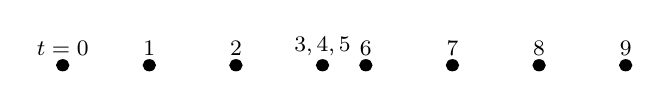
\begin{tikzpicture}[xscale=1.10,font=\footnotesize]
        \draw[fill] (-1,0) circle (2pt) node[anchor=south] {$2$};
        \draw[fill] (-2,0) circle (2pt) node[anchor=south] {$1$};
        \draw[fill] (-3,0) circle (2pt) node[anchor=south] {$t=0$};
        %% seperation
        \draw[fill] (0,0) circle (2pt) node[anchor=south] {$3,4,5$};
        \draw[fill] (0.5,0) circle (2pt) node[anchor=south] {$6$};
        \draw[fill] (1.5,0) circle (2pt) node[anchor=south] {$7$};
        \draw[fill] (2.5,0) circle (2pt) node[anchor=south] {$8$};
        \draw[fill] (3.5,0) circle (2pt) node[anchor=south] {$9$};
    \end{tikzpicture}
    \end{center}
    This diagram is most likely to describe:
    \begin{choices}
        \wrongchoice{a swimmer swimming laps.}
        \wrongchoice{an exercise on a rowing machine.}
        \wrongchoice{a person on a treadmill.}
        \wrongchoice{a tennis ball during a volley.}
      \correctchoice{a runner who tripped, fell, rose, and continued racing.}
    \end{choices}
\end{question}
}


\endinput


